%%%%%%%%%%%%%%%%%%%%%%%%%%%%%%%%%%%%%%%%%
% Beamer Presentation
% LaTeX Template
% Version 1.0 (10/11/12)
%
% This template has been downloaded from:
% http://www.LaTeXTemplates.com
%
% License:
% CC BY-NC-SA 3.0 (http://creativecommons.org/licenses/by-nc-sa/3.0/)
%
%%%%%%%%%%%%%%%%%%%%%%%%%%%%%%%%%%%%%%%%%

%----------------------------------------------------------------------------------------
%	PACKAGES AND THEMES
%----------------------------------------------------------------------------------------

\documentclass[aspectratio=169,usenames,dvipsnames]{beamer}

\usepackage[utf8]{inputenc}
\usepackage{booktabs}
\usepackage{tabularx}
\usepackage{amsmath}
\usepackage[authordate,bibencoding=auto,strict,backend=biber,natbib]{biblatex-chicago}
\addbibresource{bib.bib}
\usepackage{graphicx}
% \hypersetup{
%     colorlinks,
%     %citecolor=black,
%     linkcolor=black
% }
\usepackage{array}
\usepackage{caption}
\usepackage{threeparttable}
\usepackage{epigraph} 
\usepackage{lscape}
\usepackage{adjustbox}
\newcommand*{\Scale}[2][4]{\scalebox{#1}{\ensuremath{#2}}}%
\usepackage{import}
\newenvironment{wideitemize}{\itemize\addtolength{\itemsep}{10pt}}{\enditemize}
\usepackage{amsmath}
\usepackage{csvsimple}
\usepackage{siunitx}
\usepackage{filecontents}
\usepackage{rotating}
\usepackage{multirow}
\usepackage{amsmath}
\usepackage{subcaption}
\usepackage{appendixnumberbeamer}
\usepackage{float}
\usepackage{amsmath}
\usepackage{csvsimple}
\usepackage{hyperref}
\newtheorem{proposition}{Proposition}
\usepackage{xcolor}
\def\boxit#1#2{%
    \smash{\color{red}\fboxrule=1pt\relax\fboxsep=2pt\relax%
    \llap{\rlap{\fbox{\phantom{\rule{#1}{#2}}}}~}}\ignorespaces
}
\newenvironment{variableblock}[3]{%
  \setbeamercolor{block body}{#2}
  \setbeamercolor{block title}{#3}
  \begin{block}{#1}}{\end{block}}
\usepackage{appendixnumberbeamer}
\usepackage{tikz,pgfplots}
\usepackage{tkz-fct}
\usepackage{amsthm}
\pgfplotsset{compat=1.10}
\usepgfplotslibrary{fillbetween}
\mode<presentation> {
\AtBeginSection[]
{
    \begin{frame}
        \frametitle{Table of Contents}
        \tableofcontents[currentsection]
    \end{frame}
}
% The Beamer class comes with a number of default slide themes
% which change the colors and layouts of slides. Below this is a list
% of all the themes, uncomment each in turn to see what they look like.

\usetheme{default}
%\usetheme{AnnArbor}
%\usetheme{Antibes} -
%\usetheme{Bergen}
%\usetheme{Berkeley}
%\usetheme{Berlin}
%\usetheme{Boadilla}
%\usetheme{CambridgeUS}
%\usetheme{Copenhagen} -
%\usetheme{Darmstadt}
%\usetheme{Dresden}
%\usetheme{Frankfurt}
%\usetheme{Goettingen}
%\usetheme{Hannover}
%\usetheme{Ilmenau}
%\usetheme{JuanLesPins}
%\usetheme{Luebeck}
%\usetheme{Madrid}
%\usetheme{Malmoe}
%\usetheme{Marburg}
%\usetheme{Montpellier}
%\usetheme{PaloAlto}
%\usetheme{Pittsburgh}
%\usetheme{Rochester} -
%\usetheme{Singapore}
%\usetheme{Szeged}
%\usetheme{Warsaw}

% As well as themes, the Beamer class has a number of color themes
% for any slide theme. Uncomment each of these in turn to see how it
% changes the colors of your current slide theme.

%\usecolortheme{albatross}
%\usecolortheme{beaver}
%\usecolortheme{beetle}
%\usecolortheme{crane}
%\usecolortheme{dolphin}
%\usecolortheme{dove}
%\usecolortheme{fly}
%\usecolortheme{lily}
%\usecolortheme{orchid}
%\usecolortheme{rose}
%\usecolortheme{seagull}
%\usecolortheme{seahorse}
%\usecolortheme{whale}
%\usecolortheme{wolverine}

%\setbeamertemplate{footline} % To remove the footer line in all slides uncomment this line
%\setbeamertemplate{footline}[frame number] % To replace the footer line in all slides with a simple slide count uncomment this line
\setbeamertemplate{theorems}[numbered]
\setbeamertemplate{navigation symbols}{} % To remove the navigation symbols from the bottom of all slides uncomment this line
}
\setbeamertemplate{caption}{\raggedright\insertcaption\par}
  \setbeamertemplate{enumerate items}[default]
  %\setbeamertemplate{page number in head/foot}{\insertframenumber}
\usepackage{graphicx} % Allows including images
\usepackage{booktabs} % Allows the use of \toprule, \midrule and \bottomrule in tables
%\usepackage {tikz}
\newtheorem*{theorem*}{Theorem}
\newtheorem*{lemma*}{Lemma}
\newtheorem*{proposition*}{Proposition}
\newtheorem*{corollary*}{Corollary}
\newtheorem*{definition*}{Definition}
\DeclareMathOperator*{\argmin}{arg\,min}
\newtheorem*{assumption}{Assumption}
\usetikzlibrary {positioning}
\renewcommand{\arraystretch}{1.5}
\newcommand\hideit[1]{%
  \only<0| handout:1>{\mbox{}}%
  \invisible<0| handout:1>{#1}}
\usepackage[default]{lato}

\setbeamercolor{block body alerted}{bg=alerted text.fg!10}
\setbeamercolor{block title alerted}{bg=alerted text.fg!20}
\setbeamercolor{block body}{bg=structure!10}
\setbeamercolor{block title}{bg=structure!20}
\setbeamercolor{block body example}{bg=green!10}
\setbeamercolor{block title example}{bg=green!20}


\makeatletter
\let\save@measuring@true\measuring@true
\def\measuring@true{%
  \save@measuring@true
  \def\beamer@sortzero##1{\beamer@ifnextcharospec{\beamer@sortzeroread{##1}}{}}%
  \def\beamer@sortzeroread##1<##2>{}%
  \def\beamer@finalnospec{}%
}
\makeatother
%\usepackage {xcolor}

%----------------------------------------------------------------------------------------
%	TITLE PAGE
%----------------------------------------------------------------------------------------

\title[diss]{Lecture 17: Stock Options as Compensation} % The short title appears at the bottom of every slide, the full title is only on the title page
\author{Compensation in Organizations} % Your name
\institute[shortinst]{Jacob Kohlhepp}
\date{\today} % Date, can be changed to a custom date

\begin{document}

\begin{frame}
\titlepage % Print the title page as the first slide

\end{frame}

\begin{frame}{Beyond Salaries}
\begin{wideitemize}
    \item Salaries and bonuses are only one component of compensation.
    \item When people in the HR industry refer to total compensation they refer to salary, bonus and usually \textbf{stock options}.
    \item An estimated 9 million  US workers hold stock options.
    \item The lecture today will focus on stock options.
\end{wideitemize}
    
\end{frame}

\begin{frame}{What Are Stock Options?}
\centering
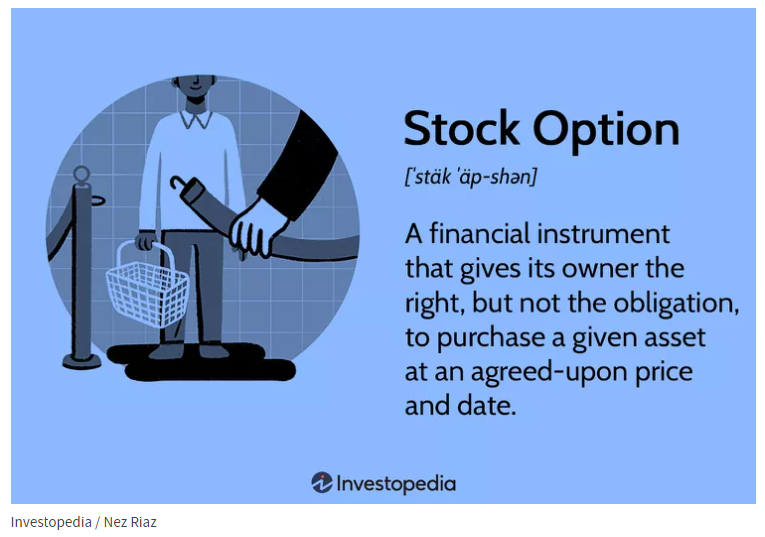
\includegraphics[width=0.8\textwidth]{pictures/stockoptions.png}

\end{frame}

\begin{frame}{What Are Employee Stock Options?}
\begin{wideitemize}
    \item Employees are allowed to buy company stock at a specified price (or at a specified discount) for a specified period of time.
    \item An employee's stock options are \textbf{vested} if the employee can exercise the option.
    \item Typically, this occurs after being with the company for a certain period of time.
    \item Employee stock options will often vest gradually.
    \item Stock options have 0 value unless the company stock rises above the specified price.
\end{wideitemize}

\end{frame}


\begin{frame}{Discussion - Reading}

\huge  Oyer and Schaefer (2005)
    
\end{frame}

\begin{frame}{Oyer and Schaefer (2005): How Large Were Stock Options in 1999}

\begin{wideitemize}
    \item Using BLS data, among firms that give out stock options, the average value granted  was \$3,331
    \begin{wideitemize}
        \item The BLS data are more representative of US firms/workers
    \end{wideitemize}
    \item Using a sample of 1000 firms with SEC filings, among firms that give out stock options, the average value granted was \$36,982.
    \begin{wideitemize}
        \item The median is \$6,551 (so there is a big right tail)
        \item These data are biased towards larger, more established firms
    \end{wideitemize}
\end{wideitemize}
    
\end{frame}
\begin{frame}{Oyer and Schaefer (2005): Three Reasons for Stock Options}
\begin{wideitemize}
    \item[1.] Incentives: linking employee compensation to firm performance
    \item[2.] Sorting: encourage people to join who have a favorable assessment of the firm.
    \item[3.] Retention: make it costly for employees to leave.
\end{wideitemize}
    
\end{frame}

\begin{frame}{Incentives}
    \begin{wideitemize}
        \item Consider our original moral hazard model with the effort-risk trade-off
        \item Oyer and Schaefer take this model and ask: how large must the return to effort be to justify using stock options as pay for performance?
        \item They account for various levels of risk aversion and different effort costs.
        \item If the return to effort is reasonable relative to the cost of effort, then incentives is a plausible story.
        \item If the return to effort is enormous relative to the cost of effort, then incentives are not a plausible story.
    \end{wideitemize}
\end{frame}

\begin{frame}{Incentives}
    \centering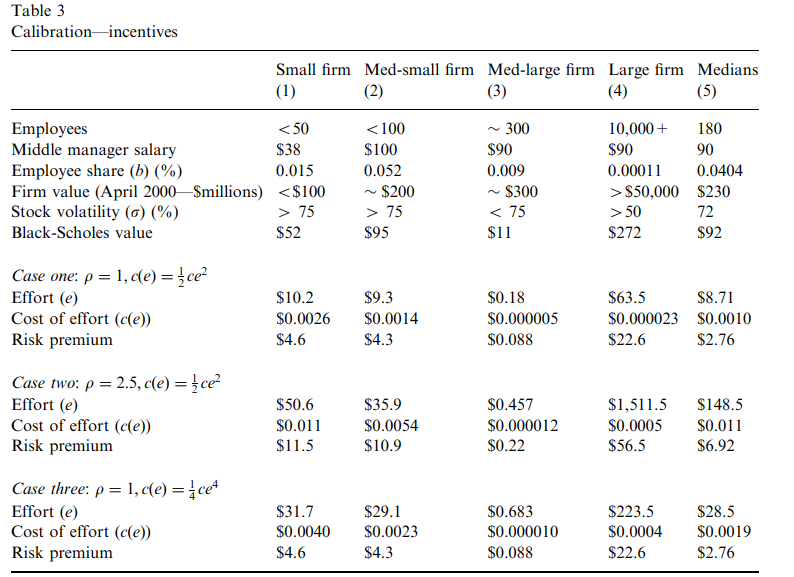
\includegraphics[width=0.7\textwidth]{pictures/incentives_stock.png}
    
    Note: all numbers are in thousands.
\end{frame}

\begin{frame}{Incentives: A Teamwork Perspective}

\begin{wideitemize}
    \item We can also think about stock options from a teamwork perspective.
    \item Suppose the stock price reflects total production of the firm.
    \item Stock represent ownership of a fraction of profit.
    \item So stock options are equivalent to a partnership with many partners.
    \item Colloquially, this is referred to as giving employees a ``stake" in the company.
\end{wideitemize}
    
\end{frame}

\begin{frame}{Incentives: A Teamwork Perspective}

\begin{wideitemize}
    \item But remember partnerships don't work in the teamwork context!
    \item Because people bare effort costs but have to share the benefits.
    \item So they free ride!
    \item Further, free riding is actually worse as the size of the team gets bigger.
    \item So stock options should be even worse than a typical partnership with 10 or fewer members.
    \item With the exception of the CEO, it is unclear if typical employees can influence stock price.
\end{wideitemize}
    
\end{frame}


\begin{frame}{Sorting}
    \begin{wideitemize}
        \item The value of stock options depends on the rate of return of the stock.
        \item If different people are more or less optimistic about the company's future, there will be different values.
        \item If people that are optimistic about the firm are more productive, stock options will sort in more productive workers.
        \item We can compare cash compensation to stock option compensation to measure this, but we need to account for risk aversion again.
        \item Oyer and Schaefer ask how much more productive do optimistic people need to be to justify using stock options?
        \item If the gap is reasonable, this is a reasonable justification for stock options.
    \end{wideitemize}
\end{frame}
\begin{frame}{Sorting}
    \centering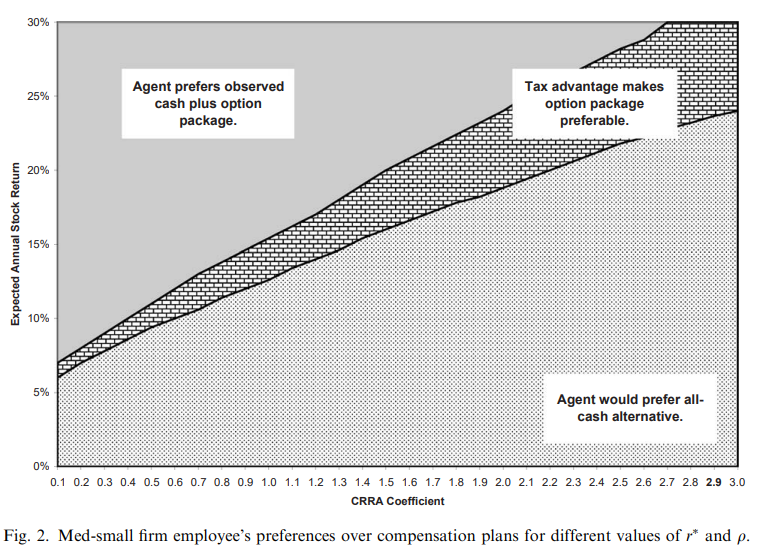
\includegraphics[width=0.8\textwidth]{pictures/sorting_stock.png}
\end{frame}

\begin{frame}{Sorting}
    \begin{wideitemize}
        \item Need employees to expect a rate of return of 25\% for employees at most firms to prefer option package.
        \item Oyer and Schaefer point out that in 1999 this was actually below the average return of these companies.
        \item using an expected return of 10\%, we need optimistic employees to be \$100 to \$50,000 more productive.
        \item The larger numbers are at larger firms.
        \item At the median firm the productivity differences are reasonable.
        \item Thus sorting might be part of the story!
    \end{wideitemize}
\end{frame}


\begin{frame}{Retention}

\begin{wideitemize}
    \item Because stock options have a vesting date, they encourage the worker to stay with the firm.
    \item Oyer and Schaefer analyze two benefits for the firm from retention:
    \begin{wideitemize}
            \item Reduced turnover costs (like HR)
            \item Reduced wage costs of matching outside offers
    \end{wideitemize}
    \item They also account for the need to compensate workers for the risk from stock options.
    \item Under high risk aversion, they find turnover costs need to be \$45,000 to justify observed stock grants
    \item Under low risk aversion, turnover costs can be close to \$0 and we can still justify observed stock grants.
    \item They conclude retention is a reasonable explanation for using stock options.
\end{wideitemize}
    
\end{frame}

\begin{frame}{Retention - Continued}
\begin{wideitemize}
    \item Professor Gong (UNC Econ) has studied the retention effects of stock options.
    \item She will present her paper in a guest lecture next class.
    \item We will briefly discuss her paper now in preparation.
    \item The content from her lecture is considered testable for the final exam!
\end{wideitemize}
    
\end{frame}

\begin{frame}{Discussion - Reading}

\huge  Gong, Zhang, Zhou (2023)
    
\end{frame}



\end{document}




